% Lineality space of the G2 Grassmannian: generator 2, pendant lengths -1,0,1,1,0,-1,0
\begingroup
\definecolor{g2TaxonBlue}{HTML}{1676A3}
\definecolor{g2TaxonYellow}{HTML}{E39A24}
\definecolor{g2HeartRed}{HTML}{D7443E}
\tikzset{
  g2tree pendant/.style={draw=black,line width=.6pt,line cap=round},
  g2tree internal/.style={draw=black,line width=2pt,line cap=round},
  g2tree vertex/.style={circle,fill=black,draw=white,line width=.4pt,inner sep=0pt,minimum size=3.8pt},
  g2tree dark/.style={fill=g2TaxonBlue,draw=white,line width=.55pt,text=white,inner sep=0pt},
  g2tree light/.style={fill=g2TaxonYellow,draw=white,line width=.55pt,text=white,inner sep=0pt},
  g2tree weight/.style={circle,fill=white,draw=none,text=black,inner sep=.15pt,minimum size=8.5pt},
  g2tree aligned pendant/.style={fill=white,text=black,inner sep=.7pt,sloped,above=1pt,font={\sffamily\fontsize{7.5}{8}\selectfont}},
  g2tree aligned internal/.style={fill=white,text=black,inner sep=1pt,sloped,above=1pt,font={\sffamily\fontsize{7.5}{8}\selectfont\bfseries}},
}
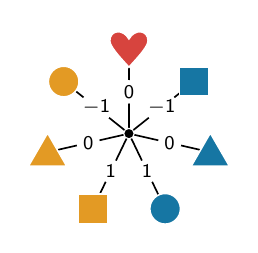
\begin{tikzpicture}[x=1.0cm,y=1.0cm,baseline=(current bounding box.center)]
\coordinate (v1) at (0.82874,0.66090);
\coordinate (v2) at (1.03342,-0.23587);
\coordinate (v3) at (0.45992,-0.95503);
\coordinate (v4) at (-0.45992,-0.95503);
\coordinate (v5) at (-1.03342,-0.23587);
\coordinate (v6) at (-0.82874,0.66090);
\coordinate (v7) at (0.00000,1.06000);
\coordinate (v8) at (0.00000,0.00000);
\draw[g2tree pendant] (v1)--(v8);
\draw[g2tree pendant] (v2)--(v8);
\draw[g2tree pendant] (v3)--(v8);
\draw[g2tree pendant] (v4)--(v8);
\draw[g2tree pendant] (v5)--(v8);
\draw[g2tree pendant] (v6)--(v8);
\draw[g2tree pendant] (v7)--(v8);
\node[g2tree weight,font={\sffamily\fontsize{7.5}{8}\selectfont}] at (0.41437,0.33045) {\(-\)1};
\node[g2tree weight,font={\sffamily\fontsize{7.5}{8}\selectfont}] at (0.51671,-0.11794) {0};
\node[g2tree weight,font={\sffamily\fontsize{7.5}{8}\selectfont}] at (0.22996,-0.47751) {1};
\node[g2tree weight,font={\sffamily\fontsize{7.5}{8}\selectfont}] at (-0.22996,-0.47751) {1};
\node[g2tree weight,font={\sffamily\fontsize{7.5}{8}\selectfont}] at (-0.51671,-0.11794) {0};
\node[g2tree weight,font={\sffamily\fontsize{7.5}{8}\selectfont}] at (-0.41437,0.33045) {\(-\)1};
\node[g2tree weight,font={\sffamily\fontsize{7.5}{8}\selectfont}] at (0.00000,0.53000) {0};
\node[g2tree vertex] at (v8) {};
\node[g2tree dark,rectangle,minimum size=3.726mm,font={\sffamily\fontsize{7.2}{7.2}\selectfont\bfseries}] at (v1) {};
\begin{scope}[shift={(v2)},scale=0.81,transform shape]
\path[fill=g2TaxonBlue,draw=white,line width=.55pt,line join=round] (0mm,3.0mm)--(-3.0mm,-2.2mm)--(3.0mm,-2.2mm)--cycle;
\end{scope}
\node[g2tree dark,circle,minimum size=3.888mm,font={\sffamily\fontsize{7.2}{7.2}\selectfont\bfseries}] at (v3) {};
\node[g2tree light,rectangle,minimum size=3.726mm,font={\sffamily\fontsize{7.2}{7.2}\selectfont\bfseries}] at (v4) {};
\begin{scope}[shift={(v5)},scale=0.81,transform shape]
\path[fill=g2TaxonYellow,draw=white,line width=.55pt,line join=round] (0mm,3.0mm)--(-3.0mm,-2.2mm)--(3.0mm,-2.2mm)--cycle;
\end{scope}
\node[g2tree light,circle,minimum size=3.888mm,font={\sffamily\fontsize{7.2}{7.2}\selectfont\bfseries}] at (v6) {};
\begin{scope}[shift={(v7)},scale=0.81,transform shape]
\path[fill=g2HeartRed,draw=white,line width=.55pt]
  (0mm,-2.7mm)..controls(-.45mm,-2.1mm)and(-3.0mm,.35mm)..(-3.0mm,1.45mm)
  ..controls(-3.0mm,3.2mm)and(-.9mm,3.4mm)..(0mm,1.75mm)
  ..controls(.9mm,3.4mm)and(3.0mm,3.2mm)..(3.0mm,1.45mm)
  ..controls(3.0mm,.35mm)and(.45mm,-2.1mm)..(0mm,-2.7mm)--cycle;
\end{scope}
\end{tikzpicture}
\endgroup
